\chapter{Технологический раздел}

В технологическом разделе выбраны и описаны средства реализации программного обеспечения и представлены детали его реализации.
В качестве языка программирования был выбран С++,~т.~к. он 
как он позволяет реализовать все алгоритмы, выбранные в результате проектирования, а также поддерживает все требуемые структуры данных. Для создания пользовательского интерфейса использовался фреймворк Qt,~т.~к. в нем присутствуют необходимые для этого инструменты, для задач визуализации --- библиотека SFML.

\section{Графический интерфейс программы}
На рисунке~\ref{fig:interface} представлен интерфейс программы. Интерфейс позволяет загрузить модель вулкана, задать скорость и направление ветра, частоту вывода кадров симуляции и перейти к окну визуализации. 

\begin{figure}[H]
	\centering
	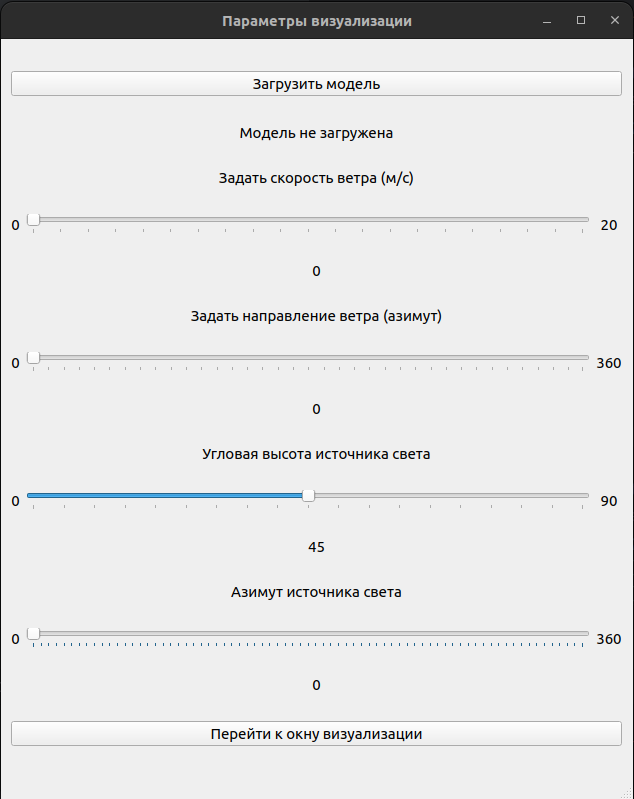
\includegraphics[width=0.8\textwidth, page=1]{assets/img/interface.png}   
	\caption{Интерфейс программы.}
	\label{fig:interface}
\end{figure}
\section{Реализация алгоритмов}

В листинге~\ref{lst:z_buf} представлен листинг функции с использованием z-буфера для визуализации модели вулкана.
\clearpage 
\begin{lstlisting}[caption={Функция использующая z-буфер для визуализации треугольника},label={lst:z_buf}]
void z_buffer(array<glm::vec3, 3> points, sf::RenderTarget &image, const sf::Color &color,
vector<float> &z_buffer) {
	if (abs(points[0].y - points[1].y) < 1e-5 && abs(points[1].y - points[2].y) < 1e-5) return;
	glm::vec<3, int, glm::defaultp> t0(round(points[0].x), round(points[0].y), round(points[0].z)),
	t1(round(points[1].x), round(points[1].y), round(points[1].z)),
	t2(round(points[2].x), round(points[2].y), round(points[2].z));
	if (t0.y > t1.y) std::swap(t0, t1);
	if (t0.y > t2.y) std::swap(t0, t2);
	if (t1.y > t2.y) std::swap(t1, t2);
	int total_height = t2.y - t0.y;
	for (int i = 0; i < total_height; i++) {
		bool second_half = i > t1.y - t0.y || t1.y == t0.y;
		int segment_height = second_half ? t2.y - t1.y : t1.y - t0.y;
		float alpha = (float) i / total_height;
		float beta = (float) (i - (second_half ? t1.y - t0.y : 0)) /
		segment_height;
		glm::vec3 A = glm::vec3(t0) + glm::vec3(t2 - t0) * alpha;
		glm::vec3 B = (second_half ? glm::vec3(t1) + glm::vec3(t2 - t1) * beta :
		glm::vec3(t0) + glm::vec3(t1 - t0) * beta);
		if (A.x > B.x) 
			std::swap(A, B);
		for (int j = round(A.x); j <= round(B.x); j++) {
			float phi = B.x == A.x ? 1. : (float) (j - A.x) / (float) (B.x - A.x);
			glm::vec3 P = glm::vec3(A) + glm::vec3(B - A) * phi;
			int idx = round(P.x + P.y * image.getSize().x);
			if (idx >= 0 && idx < z_buffer.size() && z_buffer[idx] < P.z) {
				z_buffer[idx] = P.z;
				image.draw(vector<sf::Vertex>(1, sf::Vertex(sf::Vector2f(P.x, P.y), color)).data(), 1, sf::Points);
			}
		}
	}
}
\end{lstlisting}

В листинге~\ref{lst:dens_step} приведена функция обновления распределения плотности газа.
\begin{lstlisting}[caption={Функция обновления распределения плотности дыма},label={lst:dens_step}]
void smoke::dens_step(vector<vector<vector<float>>> &x, vector<vector<vector<float>>> &x0, vector<vector<vector<float>>> &u_,
vector<vector<vector<float>>> &v_, vector<vector<vector<float>>> &w_, float d, float diff) {
	add_source(x, x0, d);
	x0.swap(x);
	diffuse(0, x, x0, diff, d);
	x0.swap(x);
	advect(0, x, x0, u_, v_, w_, d);
}
\end{lstlisting}

В листинге~\ref{lst:vel_step} представлена функция обновления поля скорости.

\begin{lstlisting}[caption={Функция обновления поля скорости},label={lst:vel_step}]
void smoke::vel_step(vector<vector<vector<float>>> &u_, vector<vector<vector<float>>> &v_, vector<vector<vector<float>>> &w_, vector<vector<vector<float>>> &v0, vector<vector<vector<float>>> &u0, vector<vector<vector<float>>> &w0, float visc, float d) {
	add_source(u_, u0, d);
	add_source(v_, v0, d);
	add_source(w_, w0, d);
	u0.swap(u_);
	diffuse(1, u_, u0, visc, d);
	v0.swap(v_);
	diffuse(2, v_, v0, visc, d);
	w0.swap(w_);
	diffuse(3, w_, w0, visc, d);
	project(u_, v_, w_, u0, v0);
	u0.swap(u_);
	v0.swap(v_);
	w0.swap(w_);
	advect(1, u_, u0, u0, v0, w0, d);
	advect(2, v_, v0, u0, v0, w0, d);
	advect(3, w_, w0, u0, v0, w0, d);
	project(u_, v_, w_, u0, v0);
}
\end{lstlisting}

В листинге~\ref{lst:advect} представлена функция вычисления адвекции.
\clearpage
\begin{lstlisting}[caption={Функция вычисления адвекции},label={lst:advect}]
void smoke::advect(int b, vector<vector<vector<float>>> &d, vector<vector<vector<float>>> &d0, vector<vector<vector<float>>> &u_, vector<vector<vector<float>>> &v_, vector<vector<vector<float>>> &w_, float dt_) {
	int i, j, i0, j0, k0, i1, j1, k1;
	float x, y, z, s0, t0, s1, t1, dt0, u1, u0;
	dt0 = dt_ * max(height, width);
	#pragma omp parallel for
	for (i = 1; i <= height; i++) {
		for (j = 1; j <= height; j++) {
			for (int k = 1; k <= width; ++k) {
				x = i - dt0 * w_[i][j][k];
				y = j - dt0 * u_[i][j][k];
				z = k - dt0 * v_[i][j][k];
				if (x < 1.5f) x = 1.5f;
				if (x > height - 0.5f) x = height - 0.5f;
				i0 = (int) x;
				i1 = i0 + 1;
				if (y < 1.5f) y = 1.5f;
				if (y > height - 0.5f) y = height - 0.5f;
				j0 = (int) y;
				j1 = j0 + 1;
				if (z < 1.5f) z = 1.5f;
				if (z > width - 0.5f) z = width - 0.5f;
				k0 = (int) z;
				k1 = k0 + 1;
				s1 = x - i0;
				s0 = 1 - s1;
				t1 = y - j0;
				t0 = 1 - t1;
				u1 = z - k0;
				u0 = 1 - u1;
				d[i][j][k] = s0 * (t0 * u0 * d0[i0][j0][k0] + t1 * u0 * d0[i0][j1][k0] + t0 * u1 * d0[i0][j0][k1] + t1 * u1 * d0[i0][j1][k1]) + s1 * (t0 * u0 * d0[i1][j0][k0] + t1 * u0 * d0[i1][j1][k0] + t0 * u1 * d0[i1][j0][k1] + t1 * u1 * d0[i1][j1][k1]);
			}
		}
	}
	set_bnd(b, d);
}
\end{lstlisting}

В листинге~\ref{lst:lin_solve} представлена функция решения СЛАУ алгоритмом на основе метода Гаусса---Зейделя.

\begin{lstlisting}[caption={Функция решения СЛАУ},label={lst:lin_solve}]
void smoke::lin_solve(int b, vector<vector<vector<float>>> &x, vector<vector<vector<float>>> &x0, float a, float c) {
	int i, j, iter;
	for (iter = 0; iter < 5; iter++) {
		for (i = 1; i <= height; i++) {
			for (j = 1; j <= height; j++) {
				for (int k = 1; k <= width; ++k) {
					x[i][j][k] = (x0[i][j][k] + a * (x[i - 1][j][k] + x[i + 1][j][k] + x[i][j - 1][k] + x[i][j + 1][k] + x[i][j][k - 1] + x[i][j][k + 1])) / c;
					
				}
			}
		}
		set_bnd(b, x);
	}
}
\end{lstlisting}

\section{Модульное тестирование}

Для модульного тестирования был использован XUnit. Тестировались критически важные функции. Покрытие составило 20,4\%. В листинге ~\ref{lst:test_voxels} приведен пример тестов для функции отрисовки вокселей.
\newpage
\begin{lstlisting}[caption={Тест для функций отрисовки вокселей},label={lst:test_voxels}]

public class VoxelGeneratorTests
{
[Fact]
public void ModelVoxel_Initialization_CorrectCenters()
{
	var bounds = new Rect3D(0, 0, 0, 10, 10, 10);
	var voxel = new VoxelGenerator.ModelVoxel(bounds, 1);
	
	Assert.Equal(new Point3D(5, 5, 5), voxel.OriginalCenter);
	Assert.Equal(new Point3D(5, 5, 5), voxel.CurrentCenter);
}
[Fact]
public void TransformContainedModels_AppliesCorrectTransformation()
{
	var bounds = new Rect3D(0, 0, 0, 10, 10, 10);
	var voxel = new VoxelGenerator.ModelVoxel(bounds, 1);
	var model = new GeometryModel3D();
	voxel.ContainedModels.Add(model);
	
	voxel.CurrentCenter = new Point3D(10, 10, 10);
	voxel.TransformContainedModels();
	
	Assert.IsType<TranslateTransform3D>(model.Transform);
}
[Fact]
public void UpdateVoxelPhysics_ChangesVoxelVelocity()
{
	var voxel = new VoxelGenerator.ModelVoxel(new Rect3D(0, 0, 0, 10, 10, 10), 1)
	{
		SpringStiffness = 0.1,
		SpringDamping = 0.9
	};
	List<VoxelGenerator.ModelVoxel> voxels = new() { voxel };
	Vector3D windForce = new(1, 0, 0);
	
	VoxelGenerator.UpdateVoxelPhysics(voxels, windForce, 0.1, false);
	
	Assert.NotEqual(new Vector3D(0, 0, 0), voxel.Velocity);
}

\end{lstlisting}

\section*{Вывод}
В данном разделе были выбраны средства реализации программного обеспечения, были проведены модульные тесты, все тесты пройдены успешно. Покрытие программы модульными тестами составило 20.4\%.
